\PassOptionsToPackage{unicode=true}{hyperref} % options for packages loaded elsewhere
\PassOptionsToPackage{hyphens}{url}
%
\documentclass[
]{article}
\usepackage{lmodern}
\usepackage{amssymb,amsmath}
\usepackage{ifxetex,ifluatex}
\ifnum 0\ifxetex 1\fi\ifluatex 1\fi=0 % if pdftex
  \usepackage[T1]{fontenc}
  \usepackage[utf8]{inputenc}
  \usepackage{textcomp} % provides euro and other symbols
\else % if luatex or xelatex
  \usepackage{unicode-math}
  \defaultfontfeatures{Scale=MatchLowercase}
  \defaultfontfeatures[\rmfamily]{Ligatures=TeX,Scale=1}
\fi
% use upquote if available, for straight quotes in verbatim environments
\IfFileExists{upquote.sty}{\usepackage{upquote}}{}
\IfFileExists{microtype.sty}{% use microtype if available
  \usepackage[]{microtype}
  \UseMicrotypeSet[protrusion]{basicmath} % disable protrusion for tt fonts
}{}
\makeatletter
\@ifundefined{KOMAClassName}{% if non-KOMA class
  \IfFileExists{parskip.sty}{%
    \usepackage{parskip}
  }{% else
    \setlength{\parindent}{0pt}
    \setlength{\parskip}{6pt plus 2pt minus 1pt}}
}{% if KOMA class
  \KOMAoptions{parskip=half}}
\makeatother
\usepackage{xcolor}
\IfFileExists{xurl.sty}{\usepackage{xurl}}{} % add URL line breaks if available
\IfFileExists{bookmark.sty}{\usepackage{bookmark}}{\usepackage{hyperref}}
\hypersetup{
  pdftitle={Homework 2 PUBH 7440},
  pdfauthor={Jake Wittman},
  pdfborder={0 0 0},
  breaklinks=true}
\urlstyle{same}  % don't use monospace font for urls
\usepackage[margin=1in]{geometry}
\usepackage{color}
\usepackage{fancyvrb}
\newcommand{\VerbBar}{|}
\newcommand{\VERB}{\Verb[commandchars=\\\{\}]}
\DefineVerbatimEnvironment{Highlighting}{Verbatim}{commandchars=\\\{\}}
% Add ',fontsize=\small' for more characters per line
\usepackage{framed}
\definecolor{shadecolor}{RGB}{248,248,248}
\newenvironment{Shaded}{\begin{snugshade}}{\end{snugshade}}
\newcommand{\AlertTok}[1]{\textcolor[rgb]{0.94,0.16,0.16}{#1}}
\newcommand{\AnnotationTok}[1]{\textcolor[rgb]{0.56,0.35,0.01}{\textbf{\textit{#1}}}}
\newcommand{\AttributeTok}[1]{\textcolor[rgb]{0.77,0.63,0.00}{#1}}
\newcommand{\BaseNTok}[1]{\textcolor[rgb]{0.00,0.00,0.81}{#1}}
\newcommand{\BuiltInTok}[1]{#1}
\newcommand{\CharTok}[1]{\textcolor[rgb]{0.31,0.60,0.02}{#1}}
\newcommand{\CommentTok}[1]{\textcolor[rgb]{0.56,0.35,0.01}{\textit{#1}}}
\newcommand{\CommentVarTok}[1]{\textcolor[rgb]{0.56,0.35,0.01}{\textbf{\textit{#1}}}}
\newcommand{\ConstantTok}[1]{\textcolor[rgb]{0.00,0.00,0.00}{#1}}
\newcommand{\ControlFlowTok}[1]{\textcolor[rgb]{0.13,0.29,0.53}{\textbf{#1}}}
\newcommand{\DataTypeTok}[1]{\textcolor[rgb]{0.13,0.29,0.53}{#1}}
\newcommand{\DecValTok}[1]{\textcolor[rgb]{0.00,0.00,0.81}{#1}}
\newcommand{\DocumentationTok}[1]{\textcolor[rgb]{0.56,0.35,0.01}{\textbf{\textit{#1}}}}
\newcommand{\ErrorTok}[1]{\textcolor[rgb]{0.64,0.00,0.00}{\textbf{#1}}}
\newcommand{\ExtensionTok}[1]{#1}
\newcommand{\FloatTok}[1]{\textcolor[rgb]{0.00,0.00,0.81}{#1}}
\newcommand{\FunctionTok}[1]{\textcolor[rgb]{0.00,0.00,0.00}{#1}}
\newcommand{\ImportTok}[1]{#1}
\newcommand{\InformationTok}[1]{\textcolor[rgb]{0.56,0.35,0.01}{\textbf{\textit{#1}}}}
\newcommand{\KeywordTok}[1]{\textcolor[rgb]{0.13,0.29,0.53}{\textbf{#1}}}
\newcommand{\NormalTok}[1]{#1}
\newcommand{\OperatorTok}[1]{\textcolor[rgb]{0.81,0.36,0.00}{\textbf{#1}}}
\newcommand{\OtherTok}[1]{\textcolor[rgb]{0.56,0.35,0.01}{#1}}
\newcommand{\PreprocessorTok}[1]{\textcolor[rgb]{0.56,0.35,0.01}{\textit{#1}}}
\newcommand{\RegionMarkerTok}[1]{#1}
\newcommand{\SpecialCharTok}[1]{\textcolor[rgb]{0.00,0.00,0.00}{#1}}
\newcommand{\SpecialStringTok}[1]{\textcolor[rgb]{0.31,0.60,0.02}{#1}}
\newcommand{\StringTok}[1]{\textcolor[rgb]{0.31,0.60,0.02}{#1}}
\newcommand{\VariableTok}[1]{\textcolor[rgb]{0.00,0.00,0.00}{#1}}
\newcommand{\VerbatimStringTok}[1]{\textcolor[rgb]{0.31,0.60,0.02}{#1}}
\newcommand{\WarningTok}[1]{\textcolor[rgb]{0.56,0.35,0.01}{\textbf{\textit{#1}}}}
\usepackage{graphicx,grffile}
\makeatletter
\def\maxwidth{\ifdim\Gin@nat@width>\linewidth\linewidth\else\Gin@nat@width\fi}
\def\maxheight{\ifdim\Gin@nat@height>\textheight\textheight\else\Gin@nat@height\fi}
\makeatother
% Scale images if necessary, so that they will not overflow the page
% margins by default, and it is still possible to overwrite the defaults
% using explicit options in \includegraphics[width, height, ...]{}
\setkeys{Gin}{width=\maxwidth,height=\maxheight,keepaspectratio}
\setlength{\emergencystretch}{3em}  % prevent overfull lines
\providecommand{\tightlist}{%
  \setlength{\itemsep}{0pt}\setlength{\parskip}{0pt}}
\setcounter{secnumdepth}{-2}
% Redefines (sub)paragraphs to behave more like sections
\ifx\paragraph\undefined\else
  \let\oldparagraph\paragraph
  \renewcommand{\paragraph}[1]{\oldparagraph{#1}\mbox{}}
\fi
\ifx\subparagraph\undefined\else
  \let\oldsubparagraph\subparagraph
  \renewcommand{\subparagraph}[1]{\oldsubparagraph{#1}\mbox{}}
\fi

% set default figure placement to htbp
\makeatletter
\def\fps@figure{htbp}
\makeatother


\title{Homework 2 PUBH 7440}
\author{Jake Wittman}
\date{2/17/2020}

\begin{document}
\maketitle

1a) From Gelman 3.2, the posterior mean given a non-informative uniform
prior on \((\mu, log \sigma)\) is

\(p(u|y_i) \sim t_{n-1}(\bar{y}, \frac{s^2}{n})\)

so \(p(u_c | y_i) \sim t_{31}(1.013, \frac{0.025^2}{32})\) and

\(p(u_t | y_i) \sim t_{35}(1.173, \frac{0.20^2}{36})\)

1b)

\begin{Shaded}
\begin{Highlighting}[]
\NormalTok{mu.c <-}\StringTok{ }\FloatTok{1.013} \OperatorTok{+}\StringTok{ }\NormalTok{(}\FloatTok{0.025}\OperatorTok{/}\KeywordTok{sqrt}\NormalTok{(}\DecValTok{32}\NormalTok{))}\OperatorTok{*}\KeywordTok{rt}\NormalTok{(}\DecValTok{1000}\NormalTok{,}\DecValTok{31}\NormalTok{)}
\NormalTok{mu.t <-}\StringTok{ }\FloatTok{1.173} \OperatorTok{+}\StringTok{ }\NormalTok{(}\FloatTok{0.20}\OperatorTok{/}\KeywordTok{sqrt}\NormalTok{(}\DecValTok{36}\NormalTok{))}\OperatorTok{*}\KeywordTok{rt}\NormalTok{(}\DecValTok{1000}\NormalTok{,}\DecValTok{35}\NormalTok{)}

\NormalTok{poster_diff <-}\StringTok{ }\NormalTok{mu.t }\OperatorTok{-}\StringTok{ }\NormalTok{mu.c}
\KeywordTok{hist}\NormalTok{(poster_diff, }\DataTypeTok{breaks =} \KeywordTok{seq}\NormalTok{(}\OperatorTok{-}\FloatTok{0.1}\NormalTok{, }\FloatTok{0.4}\NormalTok{, }\FloatTok{0.02}\NormalTok{))}
\end{Highlighting}
\end{Shaded}

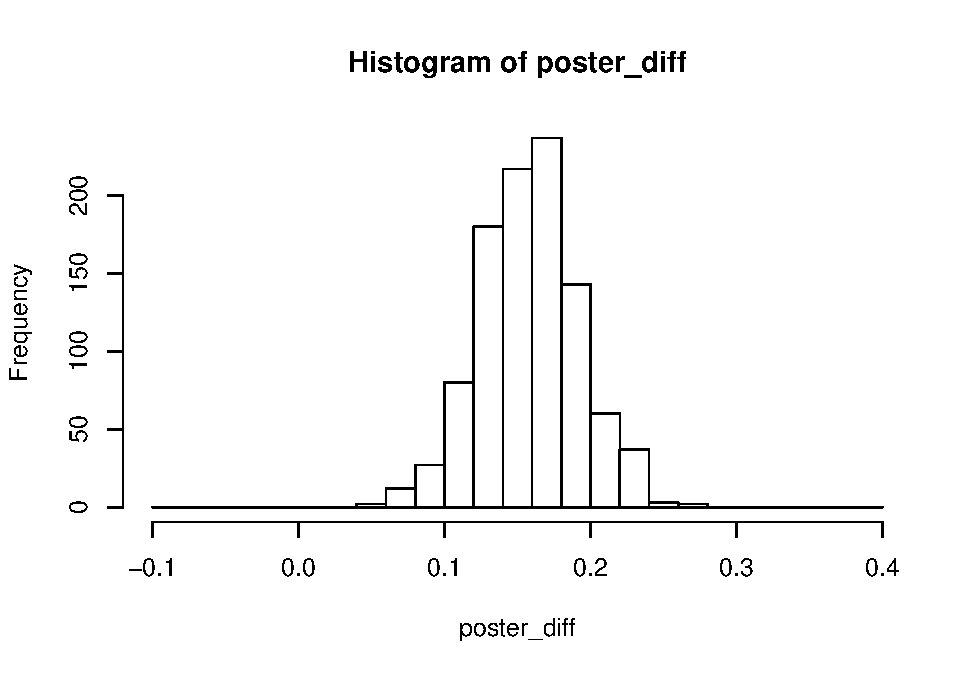
\includegraphics{hw2_files/figure-latex/unnamed-chunk-1-1.pdf}

The 95\% credible interval is {[}0.0949057, 0.2279495{]}

\begin{enumerate}
\def\labelenumi{\arabic{enumi})}
\setcounter{enumi}{1}
\item
\end{enumerate}

\(p\left(\mu, \sigma^{2} | y\right) \propto p\left(y | \mu, \sigma^{2}\right) p\left(\mu, \sigma^{2}\right)\)

\(\propto\left(\sigma^{2}\right)^{-n / 2} \exp \left(-\frac{(n-1) s^{2}+n(\mu-\bar{y})^{2}}{2 \sigma^{2}}\right) \sigma^{-1}\left(\sigma^{2}\right)^{-\left(\nu_{0} / 2+1\right)} \exp \left(-\frac{\nu_{0} \sigma_{0}^{2}+\kappa_{0}\left(\mu-\mu_{0}\right)^{2}}{2 \sigma^{2}}\right)\)

\(\propto \sigma^{-1}\left(\sigma^{2}\right)^{-\left(\left(v_{0}+n\right) / 2+1\right)} \exp \left(-\frac{\nu_{0} \sigma_{0}^{2}+(n-1) s^{2}+\frac{n \kappa_{0}\left(\bar{y}-\mu_{0}\right)^{2}}{n+\kappa_{0}}+\left(n+\kappa_{0}\right)\left(\mu-\frac{\mu_{0} \kappa_{0}+n \bar{y}}{n+\kappa_{0}}\right)^{2}}{2 \sigma^{2}}\right)\)

Because of the above,

\(\mu, \sigma^{2} | y \sim \mathrm{N}-\operatorname{Inv}-\chi^{2}\left(\frac{\mu_{0} \kappa_{0}+n \bar{y}}{n+\kappa_{0}}, \frac{\sigma_{n}^{2}}{n+\kappa_{0}} ; n+\nu_{0}, \sigma_{n}^{2}\right)\)

with

\(\sigma_{n}^{2}=\frac{\nu_{0} \sigma_{0}^{2}+(n-1) s^{2}+\frac{n \kappa_{0}\left(\bar{y}-\mu_{0}\right)^{2}}{n+\kappa_{0}}}{n+\nu_{0}}\)

3a) Stan code used to fit the models is in the code appendix at the end
of this assignment

Plots of the chains

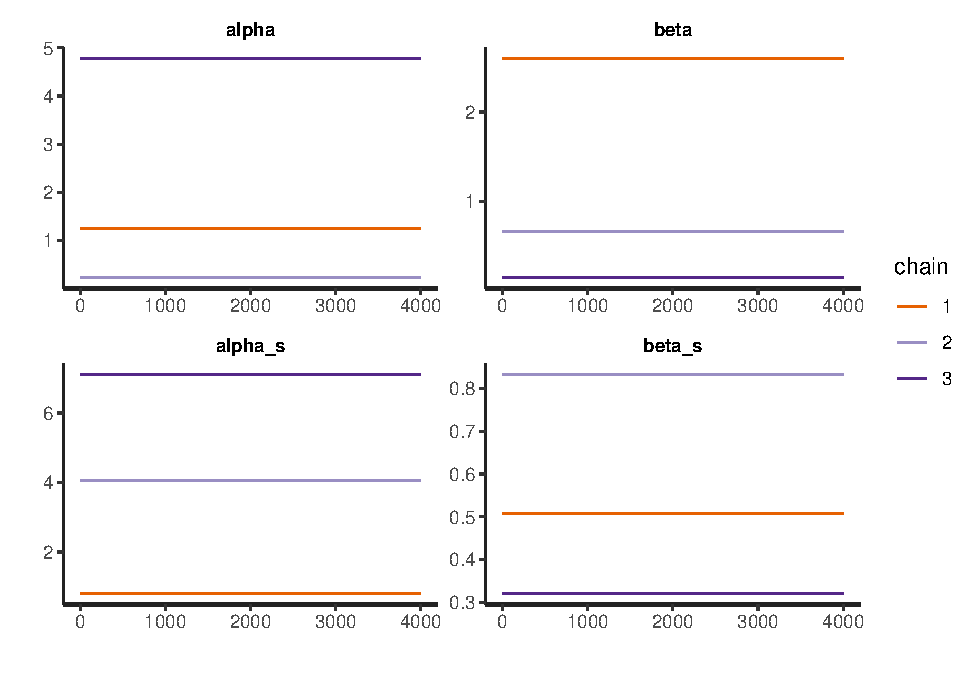
\includegraphics{hw2_files/figure-latex/unnamed-chunk-4-1.pdf}
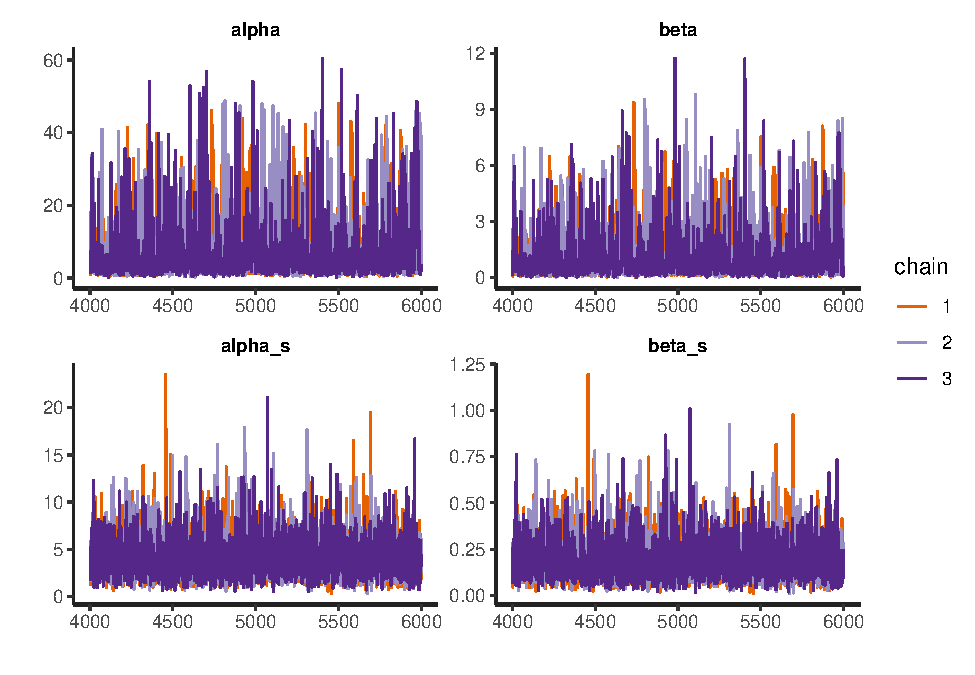
\includegraphics{hw2_files/figure-latex/unnamed-chunk-4-2.pdf}

Posterior plots for the difference in the population means and the new
predicted y value.

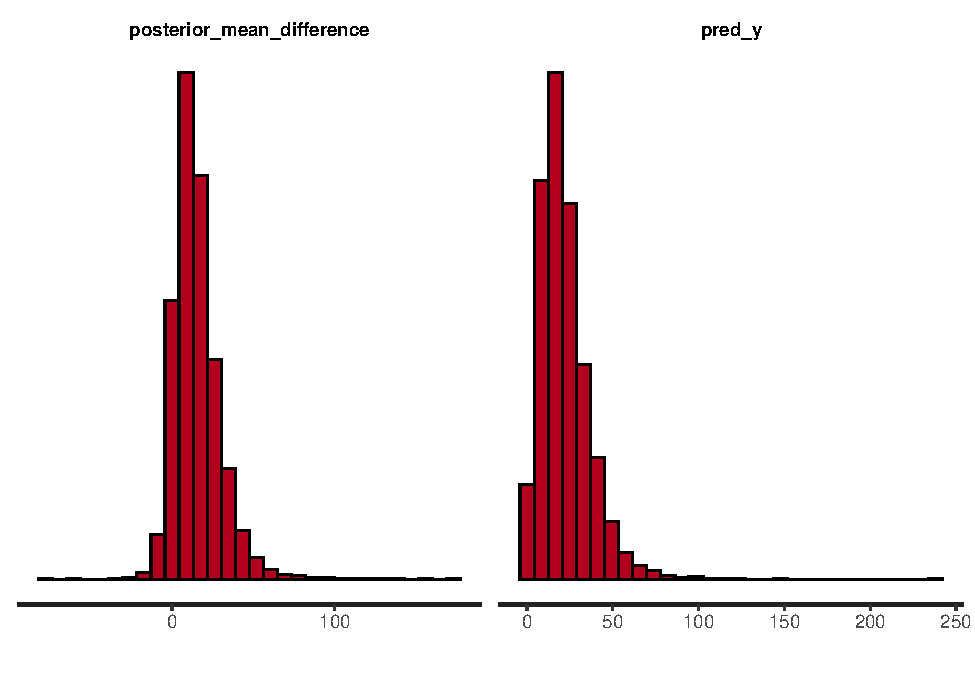
\includegraphics{hw2_files/figure-latex/unnamed-chunk-5-1.pdf}

Posterior plots with 95\% credible intervals.

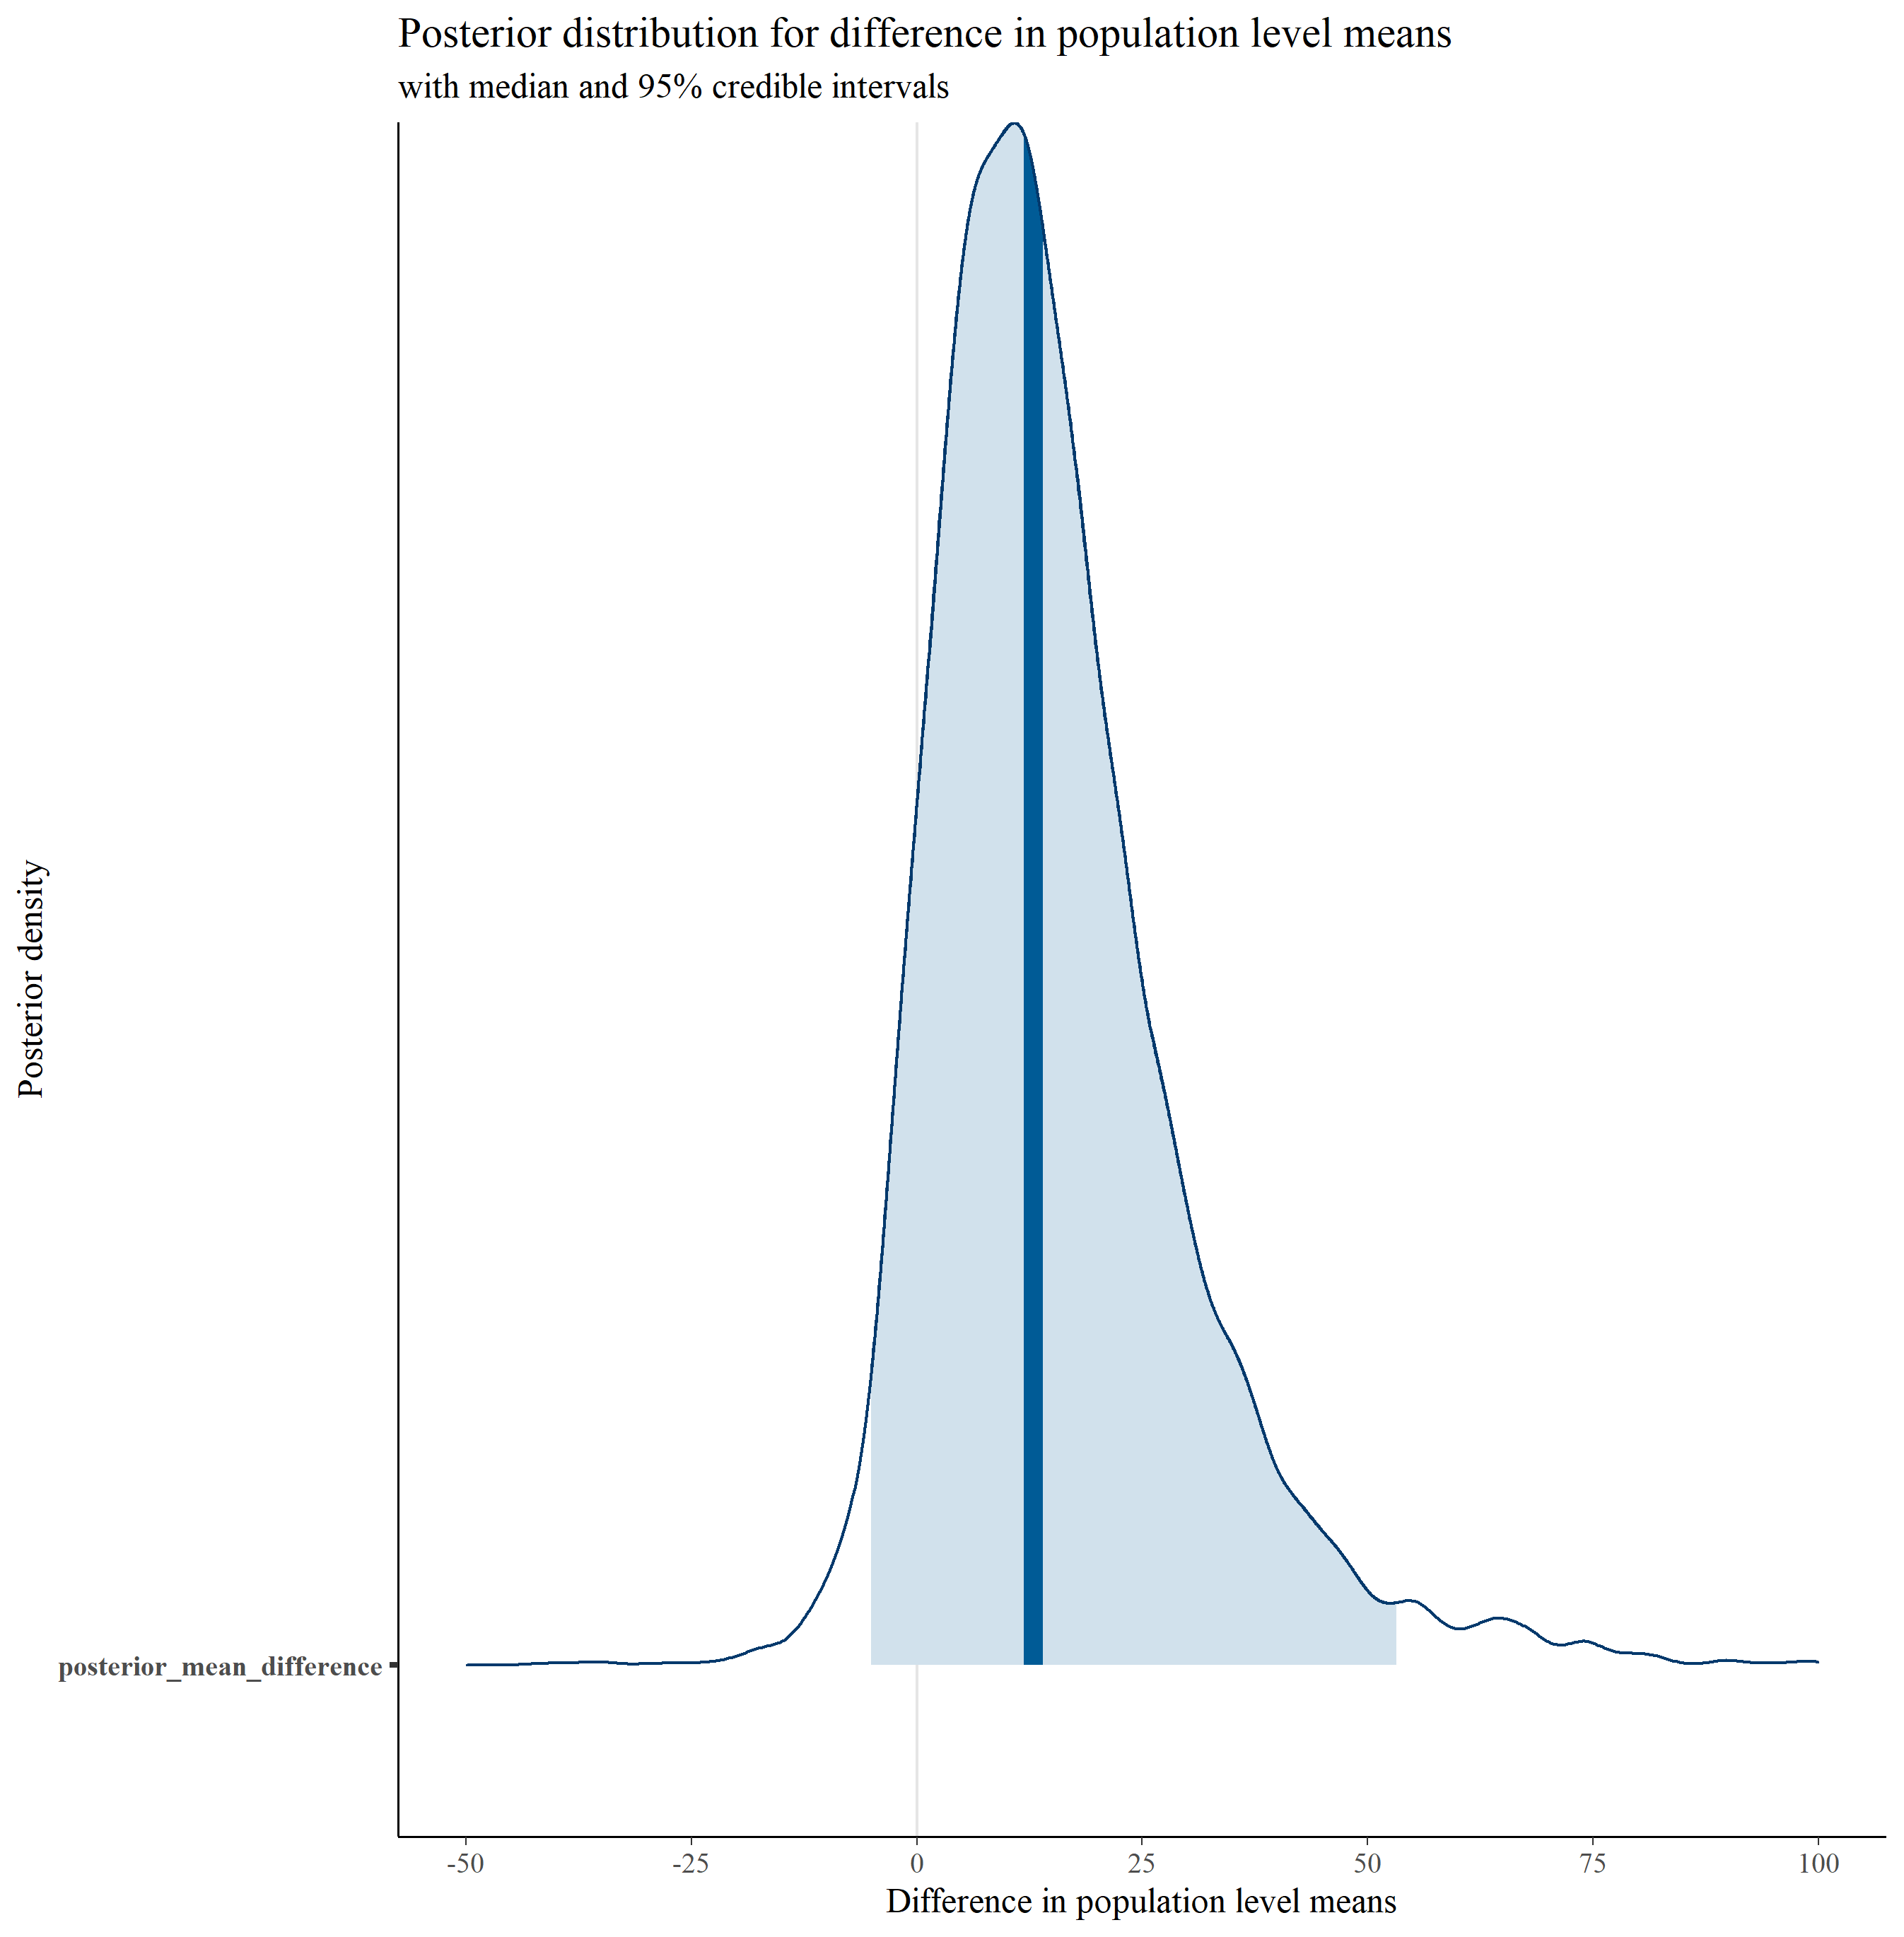
\includegraphics{C:/Users/wittm094/Google Drive/school_work/grad_school/IntroBayesianStatistics/homework/post_mean_diff.png}
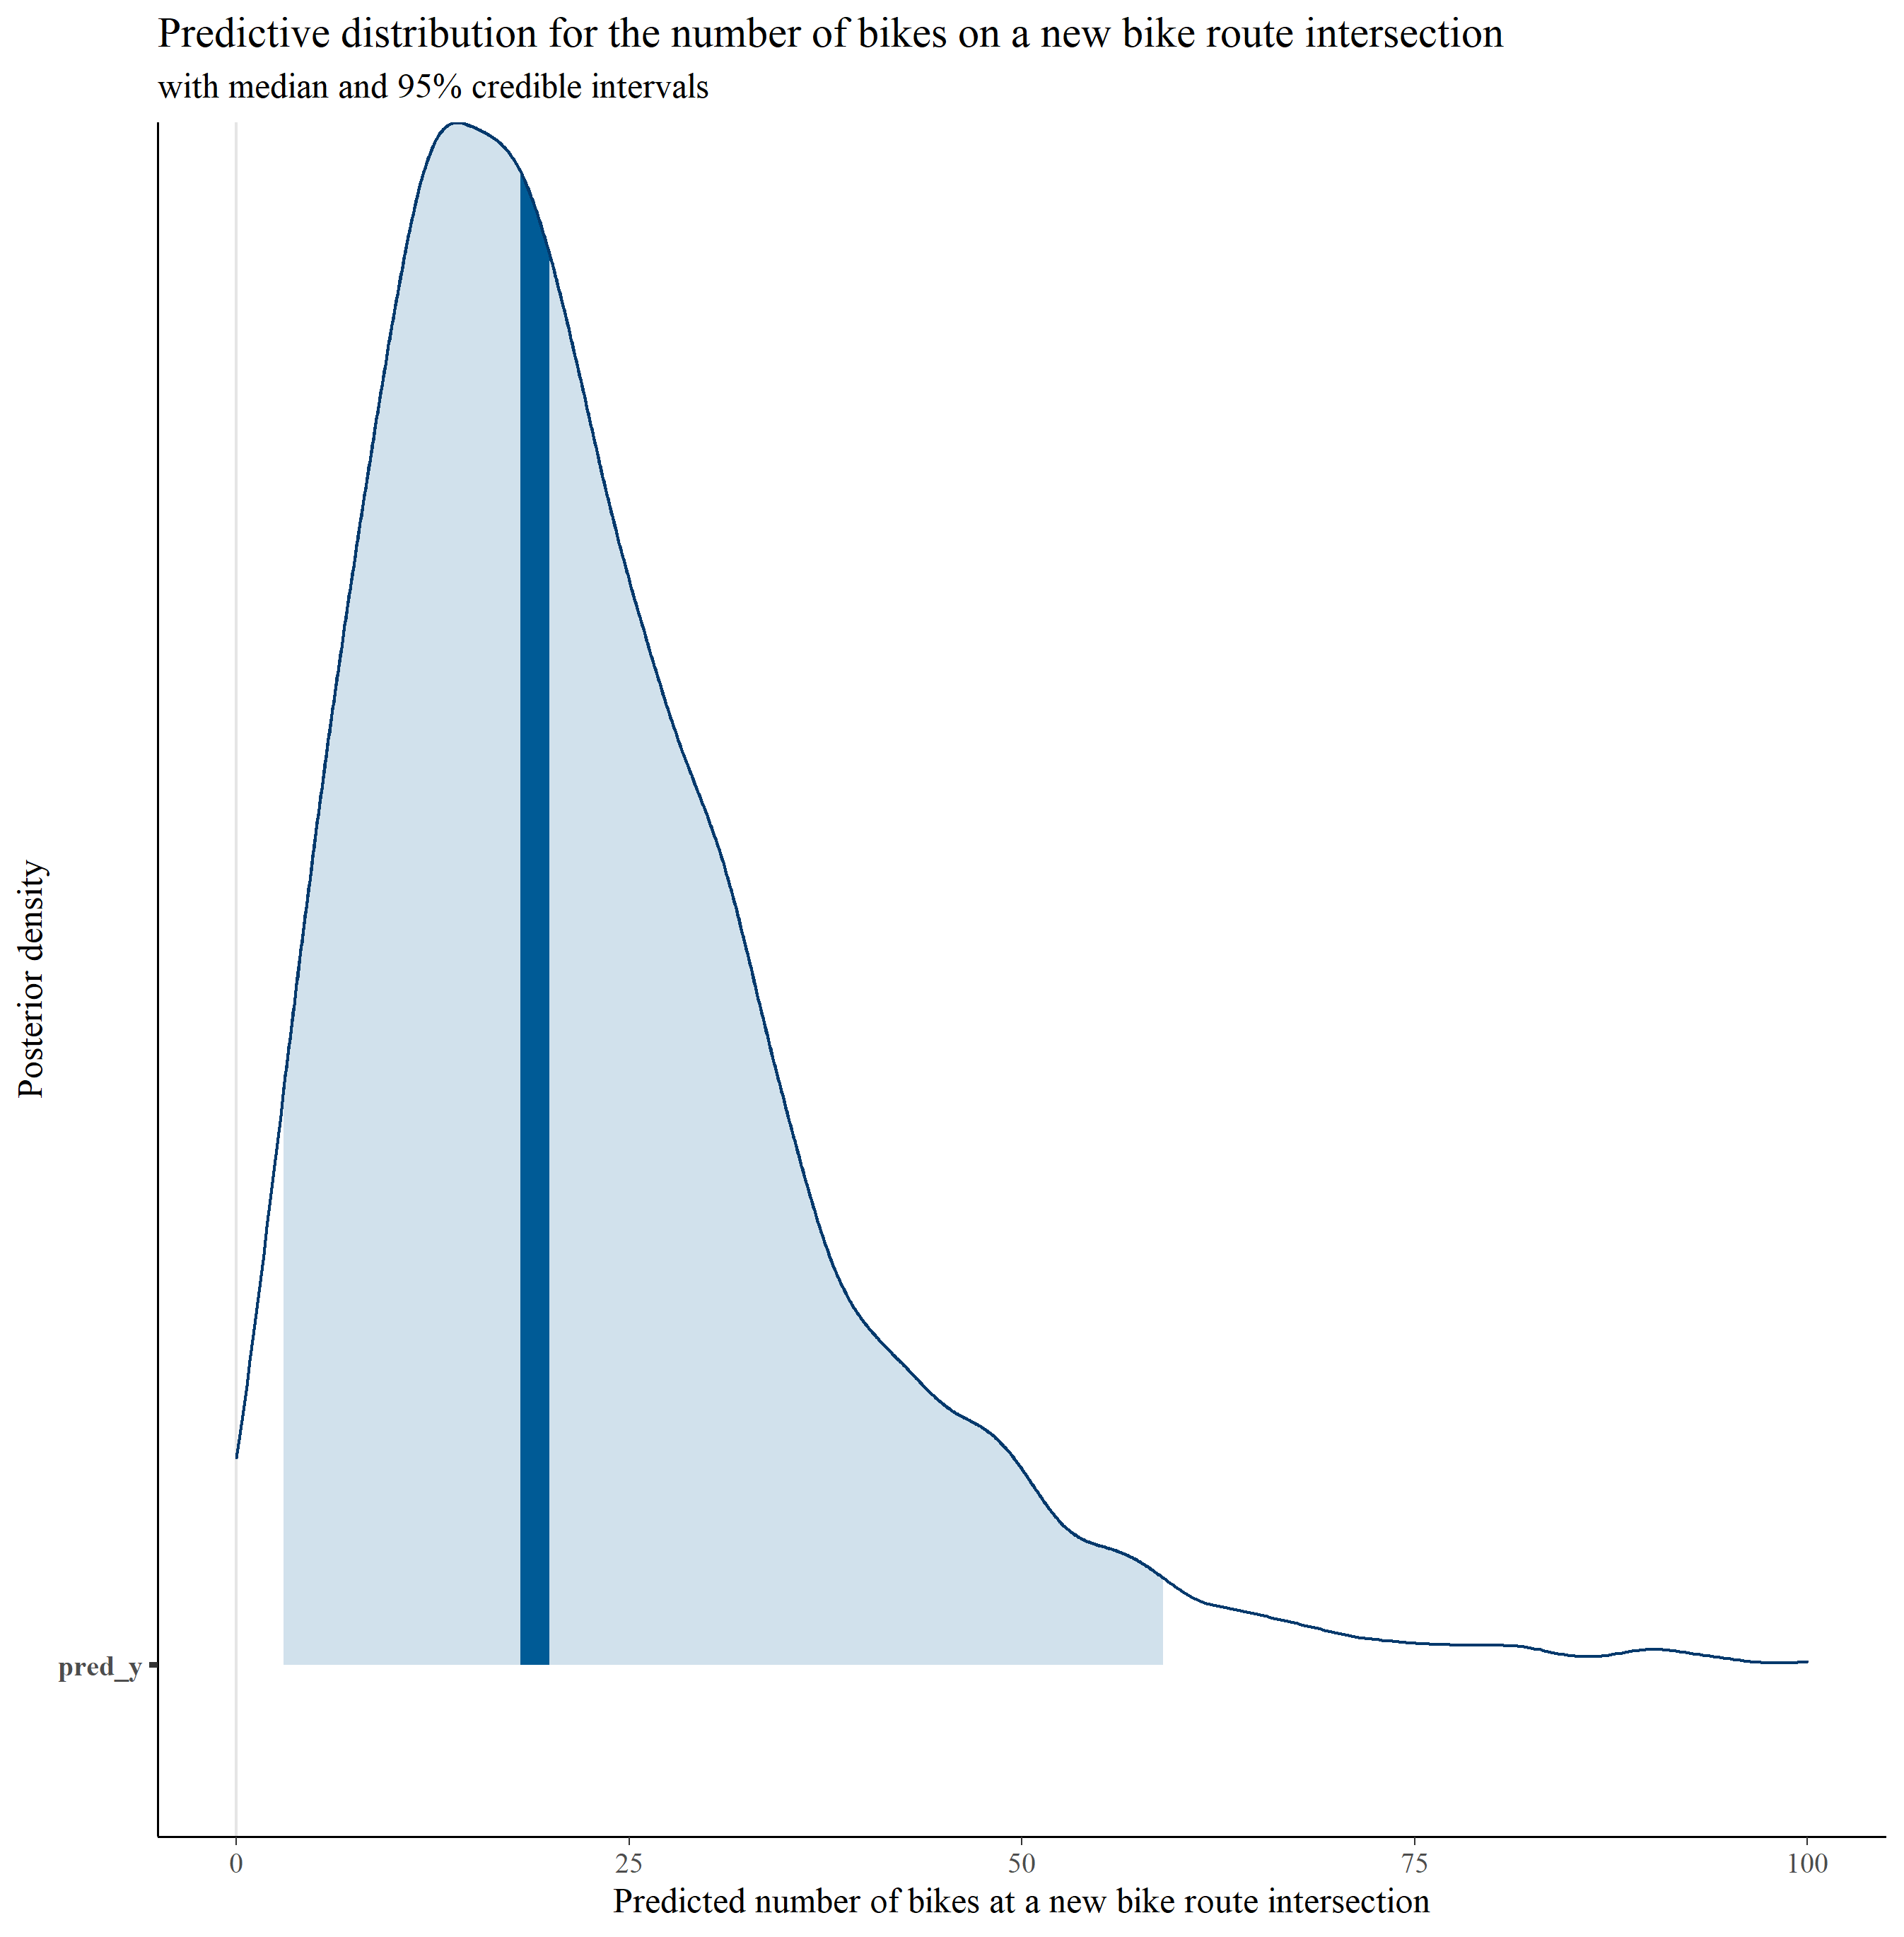
\includegraphics{C:/Users/wittm094/Google Drive/school_work/grad_school/IntroBayesianStatistics/homework/pred_y.png}

\begin{enumerate}
\def\labelenumi{\arabic{enumi})}
\setcounter{enumi}{3}
\item
\end{enumerate}

\begin{center}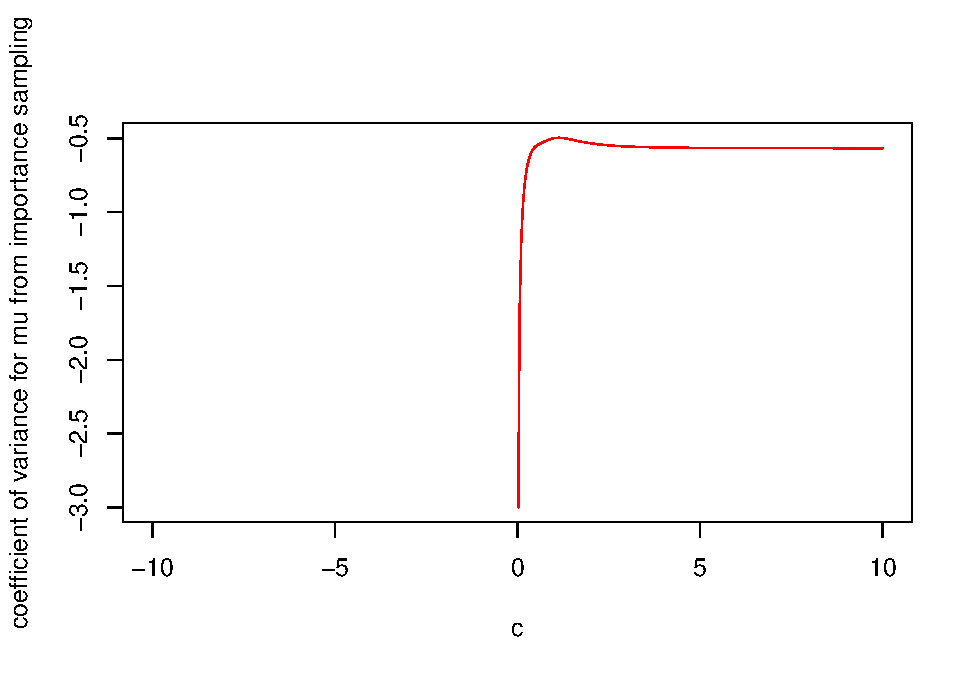
\includegraphics{hw2_files/figure-latex/unnamed-chunk-7-1} \end{center}

\begin{center}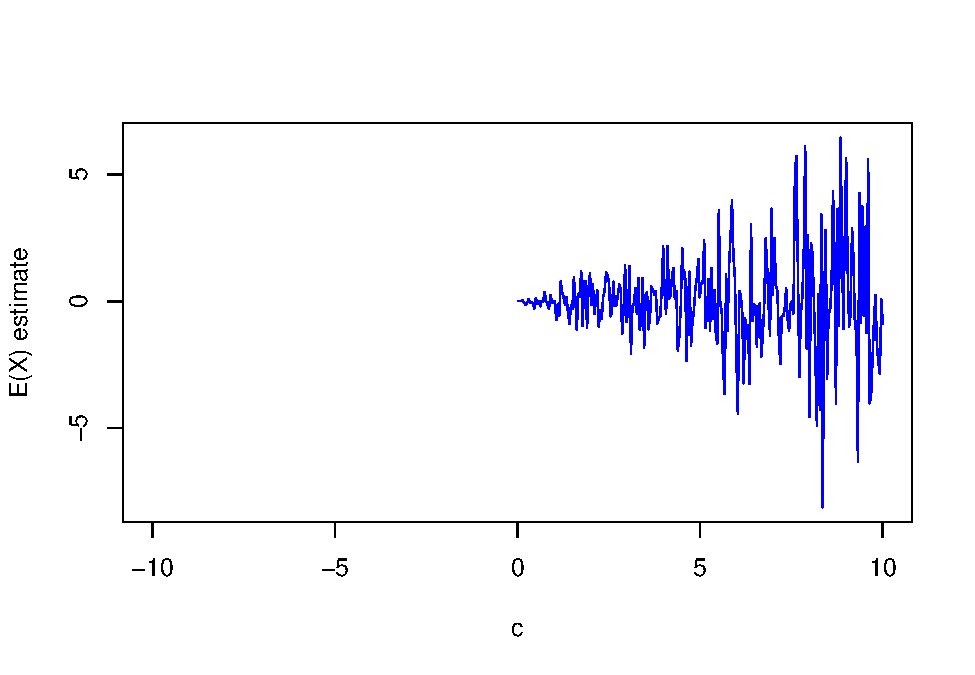
\includegraphics{hw2_files/figure-latex/unnamed-chunk-7-2} \end{center}

The final estimate for \(\mu\) from importance sampling is 0.0035294.
But I don't think I did this part right\ldots{}

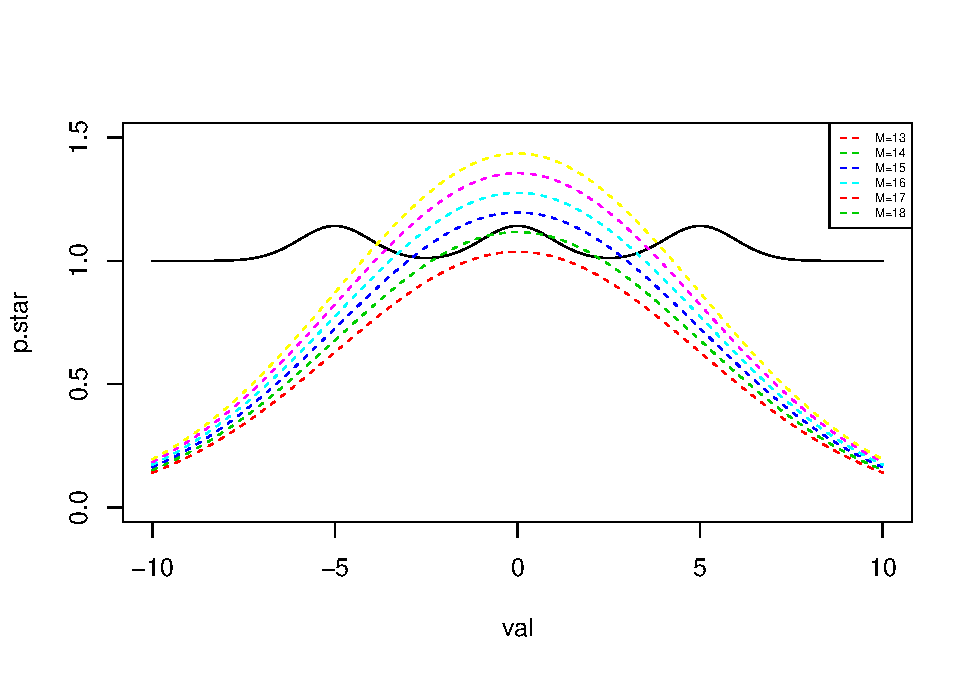
\includegraphics{hw2_files/figure-latex/unnamed-chunk-8-1.pdf}
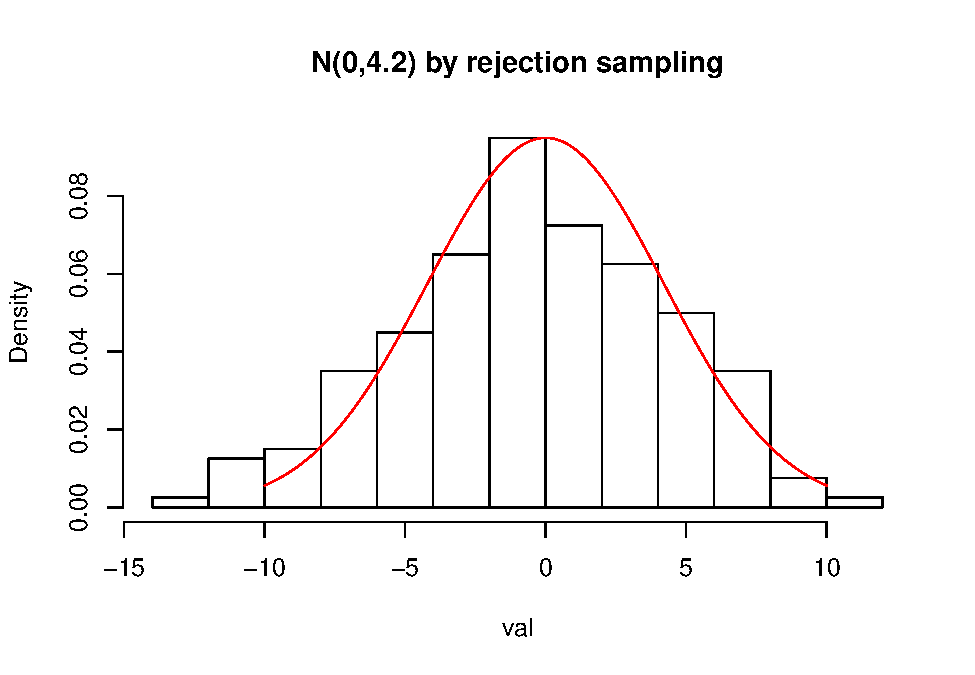
\includegraphics{hw2_files/figure-latex/unnamed-chunk-8-2.pdf}

\hypertarget{code-appendix}{%
\subsection{Code Appendix}\label{code-appendix}}

\begin{Shaded}
\begin{Highlighting}[]
\NormalTok{knitr}\OperatorTok{::}\NormalTok{opts_chunk}\OperatorTok{$}\KeywordTok{set}\NormalTok{(}\DataTypeTok{echo =} \OtherTok{FALSE}\NormalTok{)}
\NormalTok{mu.c <-}\StringTok{ }\FloatTok{1.013} \OperatorTok{+}\StringTok{ }\NormalTok{(}\FloatTok{0.025}\OperatorTok{/}\KeywordTok{sqrt}\NormalTok{(}\DecValTok{32}\NormalTok{))}\OperatorTok{*}\KeywordTok{rt}\NormalTok{(}\DecValTok{1000}\NormalTok{,}\DecValTok{31}\NormalTok{)}
\NormalTok{mu.t <-}\StringTok{ }\FloatTok{1.173} \OperatorTok{+}\StringTok{ }\NormalTok{(}\FloatTok{0.20}\OperatorTok{/}\KeywordTok{sqrt}\NormalTok{(}\DecValTok{36}\NormalTok{))}\OperatorTok{*}\KeywordTok{rt}\NormalTok{(}\DecValTok{1000}\NormalTok{,}\DecValTok{35}\NormalTok{)}

\NormalTok{poster_diff <-}\StringTok{ }\NormalTok{mu.t }\OperatorTok{-}\StringTok{ }\NormalTok{mu.c}
\KeywordTok{hist}\NormalTok{(poster_diff, }\DataTypeTok{breaks =} \KeywordTok{seq}\NormalTok{(}\OperatorTok{-}\FloatTok{0.1}\NormalTok{, }\FloatTok{0.4}\NormalTok{, }\FloatTok{0.02}\NormalTok{))}
\NormalTok{data \{}
  \OperatorTok{/}\ErrorTok{/}\StringTok{ }\NormalTok{Define data }\ControlFlowTok{in}\NormalTok{ this block}
  
  \OperatorTok{/}\ErrorTok{/}\NormalTok{data }\ControlFlowTok{for}\NormalTok{ bike route intersections}
\NormalTok{  int}\OperatorTok{<}\NormalTok{lower=}\DecValTok{0}\OperatorTok{>}\StringTok{ }\NormalTok{n_s;}\OperatorTok{/}\ErrorTok{/}\StringTok{ }\NormalTok{sample size }\ControlFlowTok{for}\NormalTok{ bike route intersections}
\NormalTok{  int}\OperatorTok{<}\NormalTok{lower=}\DecValTok{0}\OperatorTok{>}\StringTok{ }\NormalTok{y_s[n_s]; }\OperatorTok{/}\ErrorTok{/}\StringTok{ }\NormalTok{bike route data}
  
    \OperatorTok{/}\ErrorTok{/}\NormalTok{data }\ControlFlowTok{for}\NormalTok{ non}\OperatorTok{-}\NormalTok{bike route intersections}
\NormalTok{  int}\OperatorTok{<}\NormalTok{lower=}\DecValTok{0}\OperatorTok{>}\StringTok{ }\NormalTok{n;}\OperatorTok{/}\ErrorTok{/}\StringTok{ }\NormalTok{sample size }\ControlFlowTok{for}\NormalTok{ streets intersections}
\NormalTok{  int}\OperatorTok{<}\NormalTok{lower=}\DecValTok{0}\OperatorTok{>}\StringTok{ }\NormalTok{y[n]; }\OperatorTok{/}\ErrorTok{/}\StringTok{ }\NormalTok{streets data}
  
\NormalTok{\}}


\NormalTok{parameters \{}
  \OperatorTok{/}\ErrorTok{/}\StringTok{ }\NormalTok{Define parameters }\ControlFlowTok{in}\NormalTok{ this block}
  
  \OperatorTok{/}\ErrorTok{/}\StringTok{ }\NormalTok{parameters }\ControlFlowTok{for}\NormalTok{ bike route intersection}
\NormalTok{  real}\OperatorTok{<}\NormalTok{lower =}\StringTok{ }\DecValTok{0}\OperatorTok{>}\StringTok{ }\NormalTok{lambda_s[n_s]; }\OperatorTok{/}\ErrorTok{/}\NormalTok{lambda }\ControlFlowTok{for}\NormalTok{ streets}
\NormalTok{  real}\OperatorTok{<}\NormalTok{lower =}\StringTok{ }\DecValTok{0}\OperatorTok{>}\StringTok{ }\NormalTok{alpha_s; }\OperatorTok{/}\ErrorTok{/}\StringTok{ }\NormalTok{alpha }\ControlFlowTok{for}\NormalTok{ streets}
\NormalTok{  real}\OperatorTok{<}\NormalTok{lower =}\StringTok{ }\DecValTok{0}\OperatorTok{>}\StringTok{ }\NormalTok{beta_s; }\OperatorTok{/}\ErrorTok{/}\StringTok{ }\NormalTok{beta }\ControlFlowTok{for}\NormalTok{ streets}
  
    \OperatorTok{/}\ErrorTok{/}\StringTok{ }\NormalTok{parameters }\ControlFlowTok{for}\NormalTok{ non}\OperatorTok{-}\NormalTok{bike route intersection}
\NormalTok{  real}\OperatorTok{<}\NormalTok{lower =}\StringTok{ }\DecValTok{0}\OperatorTok{>}\StringTok{ }\NormalTok{lambda[n]; }\OperatorTok{/}\ErrorTok{/}\NormalTok{lambda }\ControlFlowTok{for}\NormalTok{ streets}
\NormalTok{  real}\OperatorTok{<}\NormalTok{lower =}\StringTok{ }\DecValTok{0}\OperatorTok{>}\StringTok{ }\NormalTok{alpha; }\OperatorTok{/}\ErrorTok{/}\StringTok{ }\NormalTok{alpha }\ControlFlowTok{for}\NormalTok{ streets}
\NormalTok{  real}\OperatorTok{<}\NormalTok{lower =}\StringTok{ }\DecValTok{0}\OperatorTok{>}\StringTok{ }\NormalTok{beta; }\OperatorTok{/}\ErrorTok{/}\StringTok{ }\NormalTok{beta }\ControlFlowTok{for}\NormalTok{ streets}
\NormalTok{\}}

\OperatorTok{/}\ErrorTok{/}\StringTok{ }\NormalTok{The model}
\NormalTok{model \{}
  \OperatorTok{/}\ErrorTok{/}\StringTok{ }\NormalTok{Define model }\ControlFlowTok{in}\NormalTok{ this block}
  
  \OperatorTok{/}\ErrorTok{/}\StringTok{ }\NormalTok{Model }\ControlFlowTok{for}\NormalTok{ bike route intersections}
\NormalTok{  target }\OperatorTok{+}\ErrorTok{=}\StringTok{ }\KeywordTok{gamma_lpdf}\NormalTok{(alpha_s }\OperatorTok{|}\StringTok{ }\FloatTok{0.01}\NormalTok{, }\FloatTok{0.01}\NormalTok{); }\OperatorTok{/}\ErrorTok{/}\StringTok{ }\NormalTok{gamma hyperprior on alpha }
\NormalTok{  target }\OperatorTok{+}\ErrorTok{=}\StringTok{ }\KeywordTok{gamma_lpdf}\NormalTok{(beta_s }\OperatorTok{|}\StringTok{ }\FloatTok{0.01}\NormalTok{, }\FloatTok{0.01}\NormalTok{); }\OperatorTok{/}\ErrorTok{/}\StringTok{ }\NormalTok{gamma hyperprior on beta}
\NormalTok{  target }\OperatorTok{+}\ErrorTok{=}\StringTok{ }\KeywordTok{gamma_lpdf}\NormalTok{(lambda_s }\OperatorTok{|}\StringTok{ }\NormalTok{alpha_s, beta_s); }\OperatorTok{/}\ErrorTok{/}\StringTok{ }\NormalTok{gamma prior on lambda}
\NormalTok{  target }\OperatorTok{+}\ErrorTok{=}\StringTok{ }\KeywordTok{poisson_lpmf}\NormalTok{(y_s }\OperatorTok{|}\StringTok{ }\NormalTok{lambda_s); }\OperatorTok{/}\ErrorTok{/}\StringTok{ }\NormalTok{distribution of response given lambda}
  
    \OperatorTok{/}\ErrorTok{/}\StringTok{ }\NormalTok{Model }\ControlFlowTok{for}\NormalTok{ non}\OperatorTok{-}\NormalTok{bike route intersections}
\NormalTok{  target }\OperatorTok{+}\ErrorTok{=}\StringTok{ }\KeywordTok{gamma_lpdf}\NormalTok{(alpha }\OperatorTok{|}\StringTok{ }\FloatTok{0.01}\NormalTok{, }\FloatTok{0.01}\NormalTok{); }\OperatorTok{/}\ErrorTok{/}\StringTok{ }\NormalTok{gamma hyperprior on alpha}
\NormalTok{  target }\OperatorTok{+}\ErrorTok{=}\StringTok{ }\KeywordTok{gamma_lpdf}\NormalTok{(beta }\OperatorTok{|}\StringTok{ }\FloatTok{0.01}\NormalTok{, }\FloatTok{0.01}\NormalTok{); }\OperatorTok{/}\ErrorTok{/}\StringTok{ }\NormalTok{gamma hyperprior on beta}
\NormalTok{  target }\OperatorTok{+}\ErrorTok{=}\StringTok{ }\KeywordTok{gamma_lpdf}\NormalTok{(lambda }\OperatorTok{|}\StringTok{ }\NormalTok{alpha, beta); }\OperatorTok{/}\ErrorTok{/}\StringTok{ }\NormalTok{gamma prior on lambda}
\NormalTok{  target }\OperatorTok{+}\ErrorTok{=}\StringTok{ }\KeywordTok{poisson_lpmf}\NormalTok{(y }\OperatorTok{|}\StringTok{ }\NormalTok{lambda); }\OperatorTok{/}\ErrorTok{/}\StringTok{ }\NormalTok{distribution of response given lambda}
  
\NormalTok{\}}

\NormalTok{generated quantities\{}
  \OperatorTok{/}\ErrorTok{/}\StringTok{ }\NormalTok{Define other generated quantities }\ControlFlowTok{in}\NormalTok{ this block}
  
  \OperatorTok{/}\ErrorTok{/}\StringTok{ }\NormalTok{Difference }\ControlFlowTok{in}\NormalTok{ lambdas}
\NormalTok{ real posterior_mean_difference;}
\NormalTok{ real pred_lambda;}
\NormalTok{ real pred_y;}
 
  
\NormalTok{ posterior_mean_difference =}\StringTok{ }\KeywordTok{gamma_rng}\NormalTok{(alpha_s, beta_s) }\OperatorTok{-}\StringTok{ }\KeywordTok{gamma_rng}\NormalTok{(alpha, beta);}
 
\NormalTok{ pred_lambda =}\StringTok{ }\KeywordTok{gamma_rng}\NormalTok{(alpha_s, beta_s);}
\NormalTok{ pred_y =}\StringTok{ }\KeywordTok{poisson_rng}\NormalTok{(pred_lambda);}

  
\NormalTok{\}}

\CommentTok{# Load libraries ----------------------------------------------------------}
\NormalTok{pacman}\OperatorTok{::}\KeywordTok{p_load}\NormalTok{(tidyverse,}
\NormalTok{               rstan, }
\NormalTok{               brms,}
\NormalTok{               bayesplot)}
\CommentTok{# data --------------------------------------------------------------------}
\NormalTok{intersections <-}\StringTok{ }\KeywordTok{c}\NormalTok{(}\DecValTok{1}\OperatorTok{:}\DecValTok{18}\NormalTok{)}
\NormalTok{streets <-}\StringTok{ }\KeywordTok{c}\NormalTok{(}\KeywordTok{rep}\NormalTok{(}\DecValTok{1}\NormalTok{, }\DecValTok{10}\NormalTok{), }\KeywordTok{rep}\NormalTok{(}\DecValTok{0}\NormalTok{, }\DecValTok{8}\NormalTok{))}
\NormalTok{bikes <-}\StringTok{ }\KeywordTok{c}\NormalTok{(}\DecValTok{16}\NormalTok{, }\DecValTok{9}\NormalTok{, }\DecValTok{10}\NormalTok{, }\DecValTok{13}\NormalTok{, }\DecValTok{19}\NormalTok{, }\DecValTok{20}\NormalTok{, }\DecValTok{18}\NormalTok{, }\DecValTok{17}\NormalTok{, }\DecValTok{35}\NormalTok{, }\DecValTok{55}\NormalTok{, }\DecValTok{12}\NormalTok{, }\DecValTok{1}\NormalTok{, }\DecValTok{2}\NormalTok{, }\DecValTok{4}\NormalTok{, }\DecValTok{9}\NormalTok{, }\DecValTok{7}\NormalTok{, }\DecValTok{9}\NormalTok{, }\DecValTok{8}\NormalTok{)}

\NormalTok{bike <-}\StringTok{ }\KeywordTok{data.frame}\NormalTok{(}
  \DataTypeTok{intersections =}\NormalTok{ intersections,}
  \DataTypeTok{streets =}\NormalTok{ streets,}
  \DataTypeTok{bikes =}\NormalTok{ bikes}
\NormalTok{)}

\NormalTok{bike_street <-}\StringTok{ }\NormalTok{bike }\OperatorTok\StringTok{ }\NormalTok{dplyr}\OperatorTok{::}\KeywordTok{filter}\NormalTok{(streets }\OperatorTok{==}\StringTok{ }\DecValTok{1}\NormalTok{)}
\NormalTok{bike_no_streets <-}\StringTok{ }\NormalTok{bike }\OperatorTok\StringTok{ }\NormalTok{dplyr}\OperatorTok{::}\KeywordTok{filter}\NormalTok{(streets }\OperatorTok{==}\StringTok{ }\DecValTok{0}\NormalTok{)}


\CommentTok{# Stan model --------------------------------------------------------------}
\NormalTok{bike_model <-}\StringTok{ }\NormalTok{rstan}\OperatorTok{::}\KeywordTok{stan_model}\NormalTok{(}\DataTypeTok{file =}\NormalTok{ here}\OperatorTok{::}\KeywordTok{here}\NormalTok{(}\StringTok{"homework/hw2.stan"}\NormalTok{))}
\CommentTok{# 3a ----------------------------------------------------------------------}
\KeywordTok{set.seed}\NormalTok{(}\DecValTok{1}\NormalTok{)}
\NormalTok{out_model1_streets <-}\StringTok{ }\KeywordTok{sampling}\NormalTok{(}
  \DataTypeTok{object =}\NormalTok{ bike_model,}
  \DataTypeTok{data =} \KeywordTok{list}\NormalTok{(}\DataTypeTok{y_s =}\NormalTok{ bike_street}\OperatorTok{$}\NormalTok{bikes,}
              \DataTypeTok{n_s =} \KeywordTok{nrow}\NormalTok{(bike_street),}
              \DataTypeTok{y =}\NormalTok{ bike_no_streets}\OperatorTok{$}\NormalTok{bikes,}
              \DataTypeTok{n =} \KeywordTok{nrow}\NormalTok{(bike_no_streets)),}
  \DataTypeTok{warmup =} \DecValTok{0}\NormalTok{,}
  \DataTypeTok{iter =} \DecValTok{4000}\NormalTok{, }
  \DataTypeTok{chains =} \DecValTok{3}\NormalTok{,}
  \DataTypeTok{cores =} \DecValTok{4}\NormalTok{,}
  \DataTypeTok{control =} \KeywordTok{list}\NormalTok{(}\DataTypeTok{adapt_delta =} \FloatTok{0.9}\NormalTok{),}
  \DataTypeTok{show_messages =} \OtherTok{FALSE}
\NormalTok{)}

\KeywordTok{traceplot}\NormalTok{(out_model1_streets, }\DataTypeTok{par =} \KeywordTok{c}\NormalTok{(}\StringTok{"alpha"}\NormalTok{, }\StringTok{"beta"}\NormalTok{, }\StringTok{"alpha_s"}\NormalTok{, }\StringTok{"beta_s"}\NormalTok{))}


\CommentTok{# 3b ----------------------------------------------------------------------}

\KeywordTok{set.seed}\NormalTok{(}\DecValTok{1}\NormalTok{)}
\NormalTok{out_model1_streets <-}\StringTok{ }\KeywordTok{sampling}\NormalTok{(}
  \DataTypeTok{object =}\NormalTok{ bike_model,}
  \DataTypeTok{data =} \KeywordTok{list}\NormalTok{(}\DataTypeTok{y_s =}\NormalTok{ bike_street}\OperatorTok{$}\NormalTok{bikes,}
              \DataTypeTok{n_s =} \KeywordTok{nrow}\NormalTok{(bike_street),}
              \DataTypeTok{y =}\NormalTok{ bike_no_streets}\OperatorTok{$}\NormalTok{bikes,}
              \DataTypeTok{n =} \KeywordTok{nrow}\NormalTok{(bike_no_streets)),}
  \DataTypeTok{warmup =} \DecValTok{4000}\NormalTok{,}
  \DataTypeTok{iter =} \DecValTok{6000}\NormalTok{, }
  \DataTypeTok{chains =} \DecValTok{3}\NormalTok{,}
  \DataTypeTok{cores =} \DecValTok{4}\NormalTok{,}
  \DataTypeTok{control =} \KeywordTok{list}\NormalTok{(}\DataTypeTok{adapt_delta =} \FloatTok{0.9}\NormalTok{), }
  \DataTypeTok{show_messages =} \OtherTok{FALSE}
\NormalTok{)}

\KeywordTok{traceplot}\NormalTok{(out_model1_streets, }\DataTypeTok{par =} \KeywordTok{c}\NormalTok{(}\StringTok{"alpha"}\NormalTok{, }\StringTok{"beta"}\NormalTok{, }\StringTok{"alpha_s"}\NormalTok{, }\StringTok{"beta_s"}\NormalTok{))}
\KeywordTok{stan_hist}\NormalTok{(out_model1_streets, }\DataTypeTok{pars =} \KeywordTok{c}\NormalTok{(}\StringTok{"posterior_mean_difference"}\NormalTok{, }\StringTok{"pred_y"}\NormalTok{))}


\KeywordTok{mcmc_areas}\NormalTok{(out_model1_streets,}
           \DataTypeTok{pars =} \KeywordTok{c}\NormalTok{(}\StringTok{"posterior_mean_difference"}\NormalTok{),}
           \DataTypeTok{prob =} \FloatTok{0.95}\NormalTok{) }\OperatorTok{+}
\StringTok{  }\KeywordTok{labs}\NormalTok{(}\DataTypeTok{title =} \StringTok{"Posterior distribution for difference in population level means"}\NormalTok{,}
       \DataTypeTok{subtitle =} \StringTok{"with median and 95% credible intervals"}\NormalTok{,}
       \DataTypeTok{x =} \StringTok{"Difference in population level means"}\NormalTok{,}
       \DataTypeTok{y =} \StringTok{"Posterior density"}\NormalTok{) }\OperatorTok{+}
\StringTok{  }\KeywordTok{scale_x_continuous}\NormalTok{(}\DataTypeTok{limits =} \KeywordTok{c}\NormalTok{(}\OperatorTok{-}\DecValTok{50}\NormalTok{, }\DecValTok{100}\NormalTok{),}
                     \DataTypeTok{labels =} \KeywordTok{seq}\NormalTok{(}\OperatorTok{-}\DecValTok{50}\NormalTok{, }\DecValTok{100}\NormalTok{, }\DecValTok{25}\NormalTok{),}
                     \DataTypeTok{breaks =} \KeywordTok{seq}\NormalTok{(}\OperatorTok{-}\DecValTok{50}\NormalTok{, }\DecValTok{100}\NormalTok{, }\DecValTok{25}\NormalTok{))}
  
\KeywordTok{mcmc_areas}\NormalTok{(out_model1_streets,}
           \DataTypeTok{pars =} \KeywordTok{c}\NormalTok{(}\StringTok{"diff_ys"}\NormalTok{),}
           \DataTypeTok{prob =} \FloatTok{0.95}\NormalTok{) }\OperatorTok{+}
\StringTok{  }\KeywordTok{labs}\NormalTok{(}\DataTypeTok{title =} \StringTok{"Predictive distribution for the number of bikes on a new bike route intersection"}\NormalTok{,}
       \DataTypeTok{subtitle =} \StringTok{"with median and 95% credible intervals"}\NormalTok{,}
       \DataTypeTok{x =} \StringTok{"Predicted number of bikes at a new bike route intersection"}\NormalTok{,}
       \DataTypeTok{y =} \StringTok{"Posterior density"}\NormalTok{) }\OperatorTok{+}
\StringTok{  }\KeywordTok{scale_x_continuous}\NormalTok{(}\DataTypeTok{limits =} \KeywordTok{c}\NormalTok{(}\DecValTok{0}\NormalTok{, }\DecValTok{100}\NormalTok{),}
                     \DataTypeTok{labels =} \KeywordTok{seq}\NormalTok{(}\DecValTok{0}\NormalTok{, }\DecValTok{100}\NormalTok{, }\DecValTok{25}\NormalTok{),}
                     \DataTypeTok{breaks =} \KeywordTok{seq}\NormalTok{(}\DecValTok{0}\NormalTok{, }\DecValTok{100}\NormalTok{, }\DecValTok{25}\NormalTok{))}

\CommentTok{# Question 4 ------------------------------------------------------------------}


\CommentTok{# Importance sampling ---------------------------------------------------------}
\NormalTok{posterior <-}\StringTok{ }\ControlFlowTok{function}\NormalTok{(x) \{}

\NormalTok{  post <-}\StringTok{ }\NormalTok{(}\DecValTok{1}\OperatorTok{/}\DecValTok{3}\NormalTok{)}\OperatorTok{*}\NormalTok{(}\DecValTok{1}\OperatorTok{/}\KeywordTok{sqrt}\NormalTok{(}\DecValTok{2}\OperatorTok{*}\NormalTok{pi))}\OperatorTok{*}\NormalTok{(}\KeywordTok{exp}\NormalTok{((}\OperatorTok{-}\DecValTok{1}\OperatorTok{/}\DecValTok{2}\NormalTok{)}\OperatorTok{*}\NormalTok{(x}\OperatorTok{+}\DecValTok{5}\NormalTok{)}\OperatorTok{^}\DecValTok{2}\NormalTok{) }\OperatorTok{+}\StringTok{ }\KeywordTok{exp}\NormalTok{((}\OperatorTok{-}\DecValTok{1}\OperatorTok{/}\DecValTok{2}\NormalTok{)}\OperatorTok{*}\NormalTok{x}\OperatorTok{^}\DecValTok{2}\NormalTok{) }\OperatorTok{+}\StringTok{ }\KeywordTok{exp}\NormalTok{((}\OperatorTok{-}\DecValTok{1}\OperatorTok{/}\DecValTok{2}\NormalTok{)}\OperatorTok{*}\NormalTok{(x}\DecValTok{-5}\NormalTok{)}\OperatorTok{^}\DecValTok{2}\NormalTok{))}
  \KeywordTok{return}\NormalTok{(post)}
\NormalTok{\}}


 
\CommentTok{# prep2: define the function to calculate log(weights)=log(p*(theta|x))-log(g(theta))}
\NormalTok{weight <-}\StringTok{ }\ControlFlowTok{function}\NormalTok{(mu_j, c_mean, c_sd)\{}
   
    \KeywordTok{posterior}\NormalTok{(mu_j) }\OperatorTok{-}\StringTok{ }\KeywordTok{dnorm}\NormalTok{(mu_j, }\DataTypeTok{mean =}\NormalTok{ c_mean, }\DataTypeTok{sd =}\NormalTok{ c_sd)}
\NormalTok{\}}


\NormalTok{IS <-}\StringTok{ }\ControlFlowTok{function}\NormalTok{(X, c, N) \{}
 
    \CommentTok{# first calculate all the parameters }
\NormalTok{    n <-}\StringTok{ }\KeywordTok{length}\NormalTok{(X) }
\NormalTok{    c_mean <-}\StringTok{ }\NormalTok{c }\OperatorTok{*}\StringTok{ }\DecValTok{0}
\NormalTok{    c_sd <-}\StringTok{ }\NormalTok{c }\OperatorTok{*}\StringTok{ }\FloatTok{4.2}
\NormalTok{    mu_j <-}\StringTok{ }\NormalTok{X}
    
    \CommentTok{# step 1: generate N samples from the importance function g(theta)}
\NormalTok{    theta <-}\StringTok{ }\KeywordTok{rnorm}\NormalTok{(N, c_mean, c_sd)}
    
    
    \CommentTok{# step 2: use the defined functions to calculate log of weights}
    \CommentTok{# We work in the log scale for the sake of computational stability}
\NormalTok{    lw <-}\StringTok{ }\KeywordTok{weight}\NormalTok{(mu_j, c_mean, c_sd)}
    
    
    \CommentTok{# The following step is to avoid inifite values when taking exponential of lw}
    \CommentTok{# Using the step we have weights:  w = exp(lw) = exp(w.scaled)*exp(max(lw))}
    \CommentTok{# Since w are in both the nominator and the denominator, exp(max(lw)) will be canceled out}
\NormalTok{    lw.scaled <-}\StringTok{ }\NormalTok{lw }\OperatorTok{-}\StringTok{ }\KeywordTok{max}\NormalTok{(lw)}
 

    \CommentTok{## Finally, calculate the importance sampling estimate}
\NormalTok{    theta.hat <-}\StringTok{ }\KeywordTok{mean}\NormalTok{(theta }\OperatorTok{*}\StringTok{ }\NormalTok{lw.scaled) }\OperatorTok{/}\StringTok{ }\KeywordTok{mean}\NormalTok{(lw.scaled)}

        
    \CommentTok{## Now, evaluate the importance function using the coefficient of variance}
\NormalTok{    c.v <-}\StringTok{ }\KeywordTok{sd}\NormalTok{(lw.scaled)}\OperatorTok{/}\KeywordTok{mean}\NormalTok{(lw.scaled)}
    
    
    \KeywordTok{return}\NormalTok{(}\KeywordTok{c}\NormalTok{(theta.hat,c.v))}
\NormalTok{\}}


\CommentTok{## consider a grid of c values}
\NormalTok{c.candidate <-}\StringTok{ }\KeywordTok{seq}\NormalTok{(}\OperatorTok{-}\DecValTok{10}\NormalTok{, }\DecValTok{10}\NormalTok{, }\DataTypeTok{length=}\DecValTok{500}\NormalTok{)}


\CommentTok{## specify vectors to store theta.hat and c.v for each value of c.candidate}
\NormalTok{hats <-}\StringTok{ }\KeywordTok{rep}\NormalTok{(}\OtherTok{NA}\NormalTok{, }\DecValTok{500}\NormalTok{)}
\NormalTok{cvs_hats <-}\StringTok{ }\KeywordTok{rep}\NormalTok{(}\OtherTok{NA}\NormalTok{, }\DecValTok{500}\NormalTok{)}


\CommentTok{## calculate estimate theta.hat and coef of var for each value of c.candidate}
\KeywordTok{set.seed}\NormalTok{(}\DecValTok{12345}\NormalTok{)}
\NormalTok{vals <-}\StringTok{ }\KeywordTok{seq}\NormalTok{(}\OperatorTok{-}\DecValTok{10}\NormalTok{, }\DecValTok{10}\NormalTok{, }\DataTypeTok{length.out =} \DecValTok{500}\NormalTok{)}
\ControlFlowTok{for}\NormalTok{(i }\ControlFlowTok{in} \DecValTok{1}\OperatorTok{:}\DecValTok{500}\NormalTok{) \{}

\NormalTok{    OUT <-}\StringTok{ }\KeywordTok{IS}\NormalTok{(}\DataTypeTok{X =}\NormalTok{ vals, }\DataTypeTok{c =}\NormalTok{ c.candidate[i], }\DecValTok{200}\NormalTok{)}
\NormalTok{    hats[i] <-}\StringTok{ }\NormalTok{OUT[}\DecValTok{1}\NormalTok{]}
\NormalTok{    cvs_hats[i] <-}\StringTok{ }\NormalTok{OUT[}\DecValTok{2}\NormalTok{]}
    
\NormalTok{\} }


\CommentTok{## Examine where coef. of variance is low}

\KeywordTok{plot}\NormalTok{(c.candidate, cvs_hats, }\DataTypeTok{ylab=}\StringTok{"coefficient of variance for mu from importance sampling"}\NormalTok{, }\DataTypeTok{xlab=}\StringTok{"c"}\NormalTok{, }\DataTypeTok{col=}\DecValTok{2}\NormalTok{, }\DataTypeTok{type=}\StringTok{"l"}\NormalTok{)}


\CommentTok{## target mean estimator}

\KeywordTok{plot}\NormalTok{(c.candidate, hats, }\DataTypeTok{xlab=}\StringTok{"c"}\NormalTok{, }\DataTypeTok{ylab=}\StringTok{"E(X) estimate"}\NormalTok{, }\DataTypeTok{col=}\DecValTok{4}\NormalTok{, }\DataTypeTok{type=}\StringTok{"l"}\NormalTok{)}



\KeywordTok{set.seed}\NormalTok{(}\DecValTok{12345}\NormalTok{)}
\NormalTok{N <-}\StringTok{ }\DecValTok{200}

\CommentTok{# Rejection sampling}

\NormalTok{val <-}\StringTok{ }\KeywordTok{seq}\NormalTok{(}\OperatorTok{-}\DecValTok{10}\NormalTok{,}\DecValTok{10}\NormalTok{,}\DataTypeTok{by=}\FloatTok{0.01}\NormalTok{)}
\NormalTok{p.star <-}\StringTok{ }\KeywordTok{exp}\NormalTok{(}\KeywordTok{posterior}\NormalTok{(val))}
\KeywordTok{plot}\NormalTok{(val, p.star, }\DataTypeTok{type =} \StringTok{'l'}\NormalTok{, }\DataTypeTok{ylim =} \KeywordTok{c}\NormalTok{(}\DecValTok{0}\NormalTok{,}\FloatTok{1.5}\NormalTok{), }\DataTypeTok{xlim =} \KeywordTok{c}\NormalTok{(}\OperatorTok{-}\DecValTok{10}\NormalTok{,}\DecValTok{10}\NormalTok{))}

\NormalTok{M.cand <-}\StringTok{ }\KeywordTok{c}\NormalTok{(}\DecValTok{13}\OperatorTok{:}\DecValTok{18}\NormalTok{)}
\ControlFlowTok{for}\NormalTok{(i }\ControlFlowTok{in} \DecValTok{1}\OperatorTok{:}\KeywordTok{length}\NormalTok{(M.cand))\{ }
  \KeywordTok{lines}\NormalTok{(val,}\KeywordTok{dnorm}\NormalTok{(val, }\DataTypeTok{mean =} \DecValTok{0}\NormalTok{, }\DataTypeTok{sd =} \DecValTok{5}\NormalTok{)}\OperatorTok{*}\NormalTok{M.cand[i],}\DataTypeTok{col=}\NormalTok{i}\OperatorTok{+}\DecValTok{1}\NormalTok{,}\DataTypeTok{lty=}\DecValTok{2}\NormalTok{)}
\NormalTok{\}}
\KeywordTok{legend}\NormalTok{(}\StringTok{'topright'}\NormalTok{,}\DataTypeTok{legend=}\KeywordTok{paste0}\NormalTok{(}\StringTok{'M='}\NormalTok{,}\KeywordTok{as.character}\NormalTok{(M.cand)),}\DataTypeTok{col=}\DecValTok{2}\OperatorTok{:}\DecValTok{5}\NormalTok{,}\DataTypeTok{lty=}\DecValTok{2}\NormalTok{,}\DataTypeTok{cex=}\FloatTok{0.5}\NormalTok{)}

\NormalTok{RS <-}\StringTok{ }\ControlFlowTok{function}\NormalTok{(M,N) \{}
  
\NormalTok{  val.samples <-}\StringTok{ }\OtherTok{NULL}
  
  \ControlFlowTok{while}\NormalTok{(}\KeywordTok{length}\NormalTok{(val.samples) }\OperatorTok{<}\StringTok{ }\NormalTok{N) \{}
    
\NormalTok{    val.star <-}\StringTok{ }\KeywordTok{rnorm}\NormalTok{(}\DecValTok{200}\NormalTok{, }\DataTypeTok{mean =} \DecValTok{0}\NormalTok{, }\DataTypeTok{sd =} \DecValTok{5}\NormalTok{)}
\NormalTok{    u <-}\StringTok{ }\KeywordTok{runif}\NormalTok{(}\DecValTok{1}\NormalTok{)}
\NormalTok{    ratio <-}\StringTok{ }\KeywordTok{posterior}\NormalTok{(val.star) }\OperatorTok{/}\StringTok{ }\NormalTok{(M }\OperatorTok{*}\StringTok{ }\KeywordTok{dnorm}\NormalTok{(val.star, }\DataTypeTok{mean =} \DecValTok{0}\NormalTok{, }\DataTypeTok{sd =} \DecValTok{5}\NormalTok{))}
    
    \ControlFlowTok{if}\NormalTok{(u}\OperatorTok{<}\NormalTok{ratio) val.samples <-}\StringTok{ }\KeywordTok{c}\NormalTok{(val.samples,val.star)}
\NormalTok{  \}}
  
  \KeywordTok{return}\NormalTok{(val.samples)}
\NormalTok{\}}


\NormalTok{M <-}\StringTok{ }\DecValTok{15}
\NormalTok{val.samples <-}\StringTok{ }\KeywordTok{suppressWarnings}\NormalTok{(}\KeywordTok{RS}\NormalTok{(M, N))}


\KeywordTok{hist}\NormalTok{(val.samples, }\DataTypeTok{freq =} \OtherTok{FALSE}\NormalTok{, }\DataTypeTok{main =} \StringTok{"N(0,4.2) by rejection sampling"}\NormalTok{,}\DataTypeTok{xlab =} \KeywordTok{expression}\NormalTok{(val))}
\KeywordTok{lines}\NormalTok{(val, }\KeywordTok{dnorm}\NormalTok{(val, }\DataTypeTok{mean =} \DecValTok{0}\NormalTok{, }\DataTypeTok{sd =} \FloatTok{4.2}\NormalTok{), }\DataTypeTok{col =} \DecValTok{2}\NormalTok{)}
\end{Highlighting}
\end{Shaded}

\end{document}
